\section{Notation and Definitions}

\subsection{Presburger formula\label{presburger}}

We use an EBNF (Extended Backus-Naur Form) grammar to define Presburger formulas.
\[
\begin{array}{lcl}
\pgrammar{formula} & \gets &  \pgrammar{formula} \wedge \pgrammar{formula} \\ 
        & & ~|~ \pgrammar{formula} \vee   \pgrammar{formula} \\
        & & ~|~ \neg \pgrammar{formula} 
        ~|~ \exists \pgrammar{var}. \pgrammar{formula} \\
        & & ~|~ \forall \pgrammar{var}. \pgrammar{formula}
        ~|~ \pgrammar{atom} \\
                            
\pgrammar{atom} & \gets &  \pgrammar{term} \pgrammar{relop} \pgrammar{term}
                            \\
\pgrammar{term} & \gets &     \pgrammar{numeral}
        ~|~ \pgrammar{term} + \pgrammar{term} \\
        & & ~|~ -\pgrammar{term} \\
        & & ~|~ \pgrammar{numeral} * \pgrammar{term}
        ~|~ \pgrammar{var}
                            \\
\pgrammar{relop} & \gets &    <
        ~|~ \leq
                            ~|~ =
                            ~|~ >
                            ~|~ \geq
                            \\
\pgrammar{var} & \gets &      x
                            ~|~ y
                            ~|~ z
                            ~|~ \dots
                            \\
\pgrammar{numeral} & \gets &  0
                            ~|~ 1
                            ~|~ 2
                            ~|~ \dots
                            \\
\end{array}
\]

Note that $\pgrammar{numeral} * \pgrammar{term}$ is not a general multiplication operator;
it is a shortcut for $\pgrammar{term}+\dots+\pgrammar{term}$.

Presburger arithmetic is used mainly because it is a decidable arithmetic.
That is, there exists an algorithm which decides whether an arbitrary Presburger formula is true (valid) or not, which is important for many polyhedral operations.


\subsection{Quasi-Affine Constraints}
\label{qaffine}

A \emph{quasi-affine constraint} is a constraint over integer values and integer variables involving only the operators \lstinline{+}, \lstinline{-}, $\times$, \lstinline{/}, \lstinline{mod}, \lstinline{&&}, \lstinline{||}, \lstinline{<}, \lstinline{<=}, \lstinline{>}, \lstinline{>=}, \lstinline{==}, \lstinline{!=}, and the ternary \lstinline{?:} operator, where the second argument of \lstinline{/} and \lstinline{mod} must be a (positive) integer literal, and where at
least one of the arguments of $\times$
must be a constant expression.
An example of a quasi-affine constraint for a statement in a loop nest is $10\times i+j+n>0$, where $i$ and $j$ are loop iterators and $n$ is a
\emph{symbolic constant} (i.e., a variable that has an unknown but fixed value for the duration of
an execution).  An example of a non-quasi-affine constraint is $i \times i>0$, because we require one of the arguments be a constant.


\section{Integer Sets}

An \emph{integer set} is a set of integer tuples from $\mathbb{Z}^d$ that can be specified using  affine constraints. $d$ is the dimensionality of the set (the number of integers in each tuple) and a d-tuple is represented as $(a_1, a_2, \dots, a_d)$.  An example of a set of integer tuples is:
$$\{(1,1); (2,1); (3,1); (1,2); (2,2); (3,2)\}$$

Instead of listing all the integer tuples of the set, we describe the set using affine constraints:
$$\{S(i,j): 1 \leq i \leq 3 \wedge 1 \leq j \leq 2\}$$

\noindent where $i$ and $j$ are the dimensions of the set.
The tuples of a set can optionally have a common name, such as
$S$ in this example.
Figure~\ref{fig:set} shows a graphical representation of the map $S$.

\begin{figure}[th]
  \begin{minipage}{.22\textwidth}
    \centering
    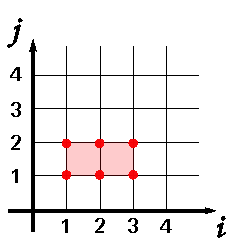
\includegraphics[scale=0.6]{figures/set.pdf}
    \captionof{figure}{Graphical representation of a set}
    \label{fig:set}
  \end{minipage}
  \begin{minipage}{.22\textwidth}
    \centering
    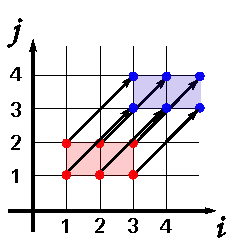
\includegraphics[scale=0.6]{figures/map.pdf}
    \captionof{figure}{Graphical representation of a map}
    \label{fig:map}
  \end{minipage}
\end{figure}

In general, an integer set has the form
$$S = \{N(\vec{s}) | f(\vec{s}, \vec{p})\}$$

\noindent with $\vec{s}$ representing the integer tuples of
the integer set ($\vec{s} \in \mathbb{Z}^d$), $N$, a common name
for all the tuples $\vec{s}$ usually used as the name of computations, $d$ the dimensionality of the set, $\vec{p} \in \mathbb{Z}^e$ a vector of $e$ parameters and $f(\vec{s}, \vec{p})$ a Presburger formula that evaluates to true, if and only if $\vec{s}$ is an element of $S$ for the given parameters $\vec{p}$.

\subsection{Relations (maps)}
A map is a relation between two integer sets.  For example
$$M = \{S1(i,j) \rightarrow S1(i+2,j+2) : 1 \leq i \leq 3 \wedge 1 \leq j \leq 2\}$$

\noindent represents a relation between two sets. The first set
is called the \emph{domain} or the \emph{source}
and the second is called the \emph{range} or the
\emph{sink}.
Figure~\ref{fig:map} shows a graphical representation of
the map $M$.


In general, a map has the form
$$M = \{A(\vec{s}) \rightarrow B(\vec{o}), (\vec{s}, \vec{o}) \in \mathbb{Z}^{d_1}\times\mathbb{Z}^{d_2} | f(\vec{s}, \vec{o}, \vec{p})\}$$

\noindent where $A(\vec{s})$ represents the domain or the
source and $B(\vec{o})$ represents the range or the sink.
$d_1$ and $d_2$ are the dimensionalities of $\vec{s}$
and $\vec{o}$, $\vec{p} \in \mathbb{Z}^e$ is a vector of $e$ parameters and $f(\vec{s}, \vec{o}, \vec{p})$ is a Presburger formula that evaluates to true if and only if there is a relation from $\vec{s}$ to $\vec{o}$ in $M$ for the given parameters
$\vec{p}$.

\section{Three-Layer IR}
\label{appendixlayers}
\subsection{Layer I: \Layerone}

The first layer is a union of \emph{computation sets} such that each computation set describes one statement in the program. Each computation set is defined as follows:
$$\{N1(\vec{s}) | f(\vec{s}, \vec{p})\} : g(N2(\vec{s}), N3(\vec{s}), ..., N4(\vec{s}))$$

\noindent where $N1(\vec{s})$ is a computation that has the name $N1$, and where $g(N2(\vec{s}), N3(\vec{s}), ..., N4(\vec{s}))$ is the expression that the computation computes and $f(\vec{s}, \vec{p})$ is a Presburger formula that evaluates to true, if and only if $\vec{s}$ is an element of $S$ for the given parameters $\vec{p}$.


\subsection{Layer II: \Layertwo}

The second layer is identical to the first layer except that computations in this layer are ordered based on their lexicographical order.

\subsection{Layer III: \Layerthree}
\label{layer3}

The third layer is a union of computation sets and a set of access relations.  The computation sets are identical to the Layer II computation sets except that new allocation/deallocation statements are added.  The set of access relations is described as follows:
$$\{N1(\vec{s}) \rightarrow B(\vec{o}), (\vec{s}, \vec{o}) \in \mathbb{Z}^{d_1}\times\mathbb{Z}^{d_2} | f(\vec{s}, \vec{o}, \vec{p})\}$$

\noindent where $N1(\vec{s})$ is a computation mapped to the buffer element $B[\vec{o}]$ and $f(\vec{s}, \vec{o}, \vec{p})$ is a Presburger formula that evaluates to true if and only if there is a relation from $\vec{s}$ to $\vec{o}$ for the given parameters $\vec{p}$.

\begin{figure}
\small

\centering\begin{lstlisting}[language=C,escapechar=@,basicstyle=\linespread{0.9}\small\ttfamily]
for (i in 0..N)
  for (j in 0..M)
    S1
    S2
\end{lstlisting}
(a) Original computation expressed as an imperative program


\begin{tabular}{c|c}
\\\hline
   \begin{tabular}{l@{\hspace{4pt}}r@{\hspace{2pt}}c@{\hspace{2pt}}c@{\hspace{2pt}}c@{\hspace{0pt}}l}
    S1: & ( & $i,$ & $j$, & $0$ & ) \\
    S2: & ( & $i$, & $j$, & 1 & ) \\
    \multicolumn{6}{c}{ (b) Sequential}
   \end{tabular}
     &  
   \begin{tabular}{l@{\hspace{4pt}}r@{\hspace{2pt}}c@{\hspace{2pt}}c@{\hspace{2pt}}c@{\hspace{0pt}}l}
    S1: & ( & $j$, & $i$, & 0 & ) \\
    S2: & ( & $j$, & $i$, & 1 & ) \\
    \multicolumn{6}{c}{ (c) Transposed}
   \end{tabular} \\\hline

    \begin{tabular}{l@{\hspace{4pt}}r@{\hspace{2pt}}c@{\hspace{2pt}}c@{\hspace{2pt}}c@{\hspace{0pt}}l}
    S1: & ( & $i$, & 0, & $j$ & ) \\
    S2: & ( & $i$, & 1, & $j$ & ) \\
    \multicolumn{6}{c}{ (d) Inner loop fission}
   \end{tabular} 
   & 
    \begin{tabular}{l@{\hspace{4pt}}r@{\hspace{2pt}}c@{\hspace{2pt}}c@{\hspace{2pt}}c@{\hspace{0pt}}l}
    S1: & ( & 0, & $i$, & $j$ & ) \\
    S2: & ( & 1, & $i$, & $j$ & ) \\
    \multicolumn{6}{c}{ (e) Outer loop fission}
   \end{tabular} \\\hline
   
    \begin{tabular}{l@{\hspace{4pt}}r@{\hspace{2pt}}c@{\hspace{2pt}}c@{\hspace{2pt}}c@{\hspace{2pt}}c@{\hspace{0pt}}l}
    S1: & (  & $i/N$, & $i\%N$, & $j$, & 0 & ) \\
    S2: & (  & $i/N$, & $i\%N$, & $j$, & 1 & ) \\
    \multicolumn{6}{c}{ (f) Loop split}
   \end{tabular} 
   &
    \begin{tabular}{l@{\hspace{4pt}}r@{\hspace{2pt}}c@{\hspace{2pt}}c@{\hspace{2pt}}c@{\hspace{2pt}}c@{\hspace{0pt}}l}
    S1: & ( & $i/N$, & $j$, & $i\%N$, & 0 & ) \\
    S2: & ( & $i/N$, & $j$, & $i\%N$, & 1 & ) \\
    \multicolumn{6}{c}{ (g) ... \& permuted}
    \end{tabular}  \\\hline
    
    \begin{tabular}{l@{\hspace{4pt}}r@{\hspace{2pt}}c@{\hspace{2pt}}c@{\hspace{2pt}}c@{\hspace{2pt}}c@{\hspace{0pt}}l}
    S1: & ( & $i\%P$ {\it (cpu)}, & $j$, & $i/P$, & 0 & ) \\
    S2: & ( & $i\%P$ {\it (cpu)}, & $j$, & $i/P$, & 1 & ) \\
    \multicolumn{6}{c}{ (h) Outer parallel }
   \end{tabular} 
   &
    \begin{tabular}{l@{\hspace{4pt}}r@{\hspace{2pt}}c@{\hspace{2pt}}c@{\hspace{2pt}}c@{\hspace{2pt}}c@{\hspace{0pt}}l}
    S1: & ( & $i$, & $j/4$, & 0, & $j\%4$ {\it (vec)} & ) \\
    S2: & ( & $i$, & $j/4$, & 1, & $j\%4$ {\it (vec)} & ) \\
    \multicolumn{6}{c}{ (i) Inner vectorized }
   \end{tabular} \\ 

\end{tabular}
 \caption{For a simple loop next with two statements, examples of different time-processor vectors leading to many possible execution arrangements. }
\label{fig:time-processor-vector}
\end{figure}

\subsection{Time-Processor Vectors}

% to map an iteration into a \processor and time order.
The {\it time-\processor vector} in Layer II is a vector indicates the logical time of execution of computations and the processor on which they should be executed.
%Computations in Layer II are represented as {\it time-\processor vectors}.
Each one of those vectors has a name associated to it (the name of the computation). $S1(0,0,0)$, $S2(0,0,1)$, $S1(i,j,0)$ and $S2(i(cpu),j,1)$ are  examples of time-\processor vectors representing computations in Layer II.
In general, the  time-\processor vector has two types of dimensions: time dimensions and \processor dimensions.
The time dimensions provide the logical order of execution of the computations while the \processor dimensions indicate on which processor the computations should be executed.
In the previous example, the first three vectors have time dimensions only, while the last vector has one space dimension.
We use a tag to indicate that a given dimension is a \processor dimension; this tag indicates mainly the type of processor to which the computations are mapped.%: cpu, gpu, node (for a distributed system), etc.

Assuming that we have two time-\processor vectors we want to know which vector among the two executes first, then all we need to do is to compare the two vectors lexicographically~\footnote{A \emph{time-\processor vector} $(i_1, \dots, i_k, \dots, i_n)$ lexicographically precedes another time-\processor vector $(i_1', \dots, i_k', \dots, i_n')$ if and only if $\exists k \in \mathbb{N}$ such that $i_1 = i_1' \wedge i_2 = i_2' \wedge \dots \wedge i_k < i_k'$}.
In the example, $S1(0,0,0]$ precedes $S2(0,0,1)$ lexicographically, so $S1(0,0,0)$ is scheduled to be executed before $S2(0,0,1)$.
The ability to add dimensions and reorder them freely enables the expression of multiple possible mappings from the original iteration space of the computations to complex execution scenarios.
Figure~\ref{fig:time-processor-vector} provides examples of different optimizations for a simple algorithm and shows the  time-\processor vectors used to express those optimizations.
Each of the dimensions of the vector can be an indexed variable, distributing the computation over that dimension or a constant providing a lexical ordering between statements. 
The algorithms will be using a custom intermediate representation within each DSL, however, we use a classical imperative language representation to describe them in this paper.
A value can be annotated by a processor type, indicating where that computation will be placed, and indicating that dimension will be run in parallel.